%\section*{Suite des exemples de la première heure}

I$_{5}$ : Soit D$_{I_{5}}$ l'ensemble des formules en logique des propositions. On commence à utiliser la logique pour parler d'elle-même\\
VAL$_{I_{5}}$(==) = "$<\equiv>$" $\rightarrow$ L'égalité est synonyme d'équivalence en logique des propositions\\
VAL$_{I_{5}}$($\leq$) = "$\models$" $\rightarrow$ Le signe d'inclusion entre les ensembles de modèles\\
Maintenant qu'on a défini la sémantique de l'ordre partiel en utilisant la notion de modèles, on peut prendre quelques exemples en raisonnant sur la logique :\\
\newline
p $\leq_{I_{5}}$ q   \hspace{1.5cm} p $\models_{I_{5}}$ q \hspace{1.5cm} $\models$ p $\Rightarrow$ q\\
\newline

I$_{6}$ : D$_{I_{6}}$ = l'ensemble des unificateurs d'un ensemble S de termes ou de formules\\
VAL$_{I_{6}}$(==) = égalité entre substitutions \{ (x$_{i}$,t$_{i}$)... \} : un ensemble de paires avec une variable et un terme\\
VAL$_{I_{6}}$($\leq$) = "moins général que"\\
\newline
Exemple: P(x,f(y)) \hspace{1cm} $\underbrace{P(x,z)}_{\sigma}$\\
$\sigma$' = $\sigma$ $\cup$ \{(z, f(y)\} donc 
$\sigma$' $\leq$ $\sigma$\\

Ces exemples montrent qu'on peut raisonner sur tout, y compris sur la logique et les algorithmes eux-mêmes, à partir du moment où on respecte les axiomes.

\section{Théorie des ensembles}
Elle sera utilisée pour la spécification des systèmes $\mathbb{Z}$.\\

\textbf{Ensemble} : on peut définir les ensembles de façon informelle (c'est-à-dire sans les axiomes) : \\
\begin{itemize}
\item Un ensemble peut être défini comme une énumération d'éléments \\
Ex: \{ 0,20,40,60,80,100 \} ou \{Mercure, Vénus, terre ..., Neptune\}
\item Il peut également être défini comme le prédicat d'un argument qui est vrai pour les membres. On appelle cette définition informelle "compréhension)". Certains langages comme Python possèdent des syntaxes particulières dédiées à la création de listes remplies par des compréhensions\\
Ex.: \{ n | n $\in$ $\mathbb{N}$ $\wedge$ $\exists$ k, k $\in$ $\mathbb{N}$ $\wedge$ 20k = n $\wedge$ 0 $\leq$ n $\leq$ 100 \} \\
\end{itemize}
La définition formelle des ensembles passe par 8 axiomes :
\\
\textbf{Axiomes} \\

\begin{itemize}
\item \textbf{Égalité} (1 ère définition) \\
A = B $\Leftrightarrow$ ($\forall$ x) (x $\in$ A $\Leftrightarrow$ x $\in$ B)\\
\item \textbf{Ensemble vide} (sans éléments)\\
$\emptyset$ = \{x $\vert$ x $\neq$ x\}\\
\item \textbf{Ensemble universel} (tous les éléments du domaine)\\
$\mathcal{U}$ (par exemple: $\mathbb{N}$, $\mathbb{R}$, $\mathbb{Z}$)\\
\item \textbf{Sous-ensemble}\\
A $\subseteq$ B $\Leftrightarrow$ ($\forall$ x) (x $\in$ A $\Rightarrow$ x $\in$ B)\\
A $\nsubseteq$ B $\Leftrightarrow$ $\neg$(A $\subseteq$ B)\\
A $\subset$ B $\Leftrightarrow$ A $\subseteq$ B $\wedge$ A $\neq$ B\\
\item \textbf{Construction de sous ensemble} \\
A $\subseteq$ B $\Leftrightarrow$ (x $\in$ A $\Leftrightarrow$ x $\in$ B $\wedge$ $\varphi$(x))\\
On va ici prendre des éléments de B tels que $\varphi$(x) est vrai, et les mettre dans A. C'est un peu une formulation de la notion de compréhension.\\ 
\item \textbf{Propriétés}\\
$\emptyset$ $\subseteq$ A\\
A $\subseteq$ A\\
A $\subseteq$ B $\wedge$ B $\subseteq$ C $\Rightarrow$ A $\subseteq$ C \\
\item \textbf{Égalité} (2e définition)\\
(A = B) $\Leftrightarrow$ (A $\subseteq$ B) $\wedge$ (B $\subseteq$ A)\\
\item \textbf{Taille d'un ensemble} 
    \begin{itemize}
    \item Prédicat à 2 arguments\\
    \#(A,n) \\
    \#$\emptyset$ = 0  $\rightarrow$ \#($\emptyset$, 0) 
    \item $\mathbb{P}$A = \{a $\vert$ a $\subseteq$ A\} (prédicat à 2 arguments)\\
    \#$\mathbb{P}$A = 2$^{\#A}$ \\
    \end{itemize}
\end{itemize}

\textbf{Spécification formelle des systèmes avec l'approche $\mathbb{Z}$} \\
\newline
Cette approche est "Orientée modèle" : On ne donne pas que des équations, mais aussi des structures\\
\newline
\underline{Deux concepts en $\mathbb{Z}$}: \\

Types:\\
\begin{itemize} 
\item Types génériques (ensembles): par exemple : Book, Location
\item Types énumérés: par exemple : Statuts := $\underbrace{In}_{Dans \hspace{0.1cm} la \hspace{0.1cm} bibliothèque, \hspace{0.1cm} disponible}$ $\vert$ $\overbrace{Out}^{Prêté}$ $\vert$ $\underbrace{Ref}_{Livre \hspace{0.1cm} de \hspace{0.1cm} référence}$ \\
\end{itemize}

Schémas:\\
\begin{itemize}
\item État du système : $\rightarrow$ logique des prédicats
\item Comportement actions : préconditions et posconditions $\rightarrow$ également logique des prédicats\\
\end{itemize}

\underline{Exemple d'un état} \\
\newline
\begin{center}
\newcolumntype{M}[1]{>{\raggedright}m{#1}}
	\begin{tabular}{|l|M{7cm}|}
    	\hline
    	nom & \hspace{2cm} LIB\_STOCK \tabularnewline
    	\hline
    	signature & stock\\ on\_loan\\ on\_shelf\\ ref\_coll : $\mathbb{F}$ Book  \tabularnewline
    	\hline
    	prédicat & stock = on\_loan $\cup$ on\_shelf\\ on\_loan $\cap$ on\_shelf = $\emptyset$\\ ret\_call $\subseteq$ on\_shelf \tabularnewline
    	\hline
 	\end{tabular}
\end{center}
\vspace{10 mm}
$\mathbb{F}$ Book représente un sous-ensemble fini de l'ensemble Book.\\
\newline
\underline{Exemple du comportement}\\
\begin{itemize}
\item Il y a un "avant" et un "après"\\
Les variables "avant", on les écrit normalement (sans rien changer) alors qu'on ajoute une apostrophe aux variables "après" pour pouvoir les distinguer. Ex.: Stock et Stock'
\item Une exécution est une séquence d'états\\
\newline
\begin{center}
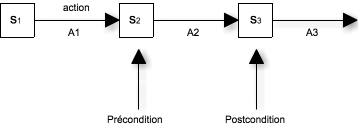
\includegraphics[scale=0.5]{images/14_sequence.png} 
\end{center}
\item Notation $\mathbb{Z}$ \\
$\Delta$ Lib\_Stock $\stackrel{\Delta}{=}$ Lib\_Stock $\wedge$ Lib\_Stock'\\
$\equiv$ Lib\_Stock $\stackrel{\Delta}{=}$ Lib\_Stock $\wedge$ (Lib\_Stock' $\vert$ Lib\_Stock = Lib\_Stock')\\
Cette deuxième ligne d'exemple veut dire la même chose, mais dans la condition où Lib\_stock n'a pas changé.\\
\newline

\begin{center}
\newcolumntype{M}[1]{>{\raggedright}m{#1}}
	\begin{tabular}{|l|M{7cm}|}
    	\hline
    	nom & \hspace{2cm} ADD\_STOCKo \tabularnewline
    	\hline
    	signature & $\Delta$ lib\_stock\\ new ? : $\mathbb{F}$  Book \tabularnewline
    	\hline
    	prédicat & new ? $\neq$ $\emptyset$ $\rightarrow$ précondition\\ new ? $\wedge$ stock = $\emptyset$ $\rightarrow$ précondition\\ stock' = stock $\cup$ new ? $\rightarrow$ postcondition\\ on\_loan' = on\_loan $\rightarrow$ postcondition\tabularnewline
    	\hline
 	\end{tabular}

\end{center}
\vspace{10 mm}

Le "?" signifie qu'il s'agit d'une entrée.\\
On peut déduire de ces prédicats que new? sera dans on\_shelf.

\item Si la ou les préconditions ne sont pas satisfaites, on aura des erreurs que l'on devra corriger via la gestion d'erreurs. Si les préconditions n'échouent jamais, on a affaire à une opération totale.\\

Exemple d'opération totale :\\

ADD\_STCK = AdDD\_STCKo $\cup$ ERRONEOUS\_NEW\_STOCK

\begin{center}
\newcolumntype{M}[1]{>{\raggedright}m{#1}}
	\begin{tabular}{|l|M{7cm}|}
    	\hline
    	nom & \hspace{1cm}ERRONEOUS\_NEW\_STOCK \tabularnewline
    	\hline
    	signature & $\equiv$ lib\_stock\\ new ? : \# Book\\ rep! : Report \tabularnewline
    	\hline
    	prédicat & (new ? = $\emptyset$ $\cup$ new ? $\cap$ stock $\wedge$ $\emptyset$) ... $\rightarrow$ préconditions\\ rep ! = "Attention stock problem" \tabularnewline
    	\hline
 	\end{tabular}

\end{center}
\vspace{10 mm}
Le "!" signifie qu'il s'agit d'une sortie.\\


\end{itemize}
